


\section{Administration}
\label{sec:adminPrensentation}
\todo{Teksten på siden er copyet fra implementationen og skal rettes til}
\todo{Der skal indsæættes SS af edit, og group list. Måske også group members list.}
\todo{Kig evt. på billedet i ovenstaaende section, hvis du syntes det er grimt må du gerne lave det om}
This section presents the system as seen and used by the administrative personnel.

can be accessed through the site administration menu as seen in \figref{fig:navigation}.

\begin{figure}[htb]
	\centering
		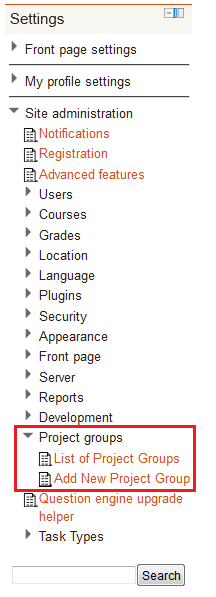
\includegraphics[scale=0.75]{images/admin-navigation.png}
	\morscaption{The settings block, which contains the site administration menu} 
	\label{fig:navigation}
\end{figure}

From here we provide a link to a list of all project groups and a link to a page, from where a new project group can be created.
The page with the list of all project groups has a table with three columns: Short name, Full name, and Actions.
As the name indicates Short name is a short name for a group. 
The Short name also serves as a link to the project group page described in \secref{sub:page}.
In the Actions column there are links to delete and edit the project group.